\section{Results}
\label{sec:results}

\subsection{Attack Success Rates}
\label{sec:asr_results}

\tabref{tab:asr} presents the attack success rates across all conditions and models.
Context manipulation CoT is the clear outlier: it achieves 20.0\% \asr on \gptmini and 7.5\% on \gptfour, substantially exceeding the direct baseline in both cases.
All other conditions remain within the confidence interval of the direct baseline.

\begin{table}[t]
    \centering
    \caption{Attack success rates (ASR) by prompting condition and model. Values show ASR with 95\% Clopper-Pearson confidence intervals in brackets. Best (highest) ASR per model in \textbf{bold}. $N = 80$ harmful behaviors per condition.}
    \resizebox{\textwidth}{!}{%
    \begin{tabular}{@{}lccccc@{}}
        \toprule
        \textbf{Model} & \textbf{Direct} & \textbf{\simplecot} & \textbf{\snowball} & \textbf{\contextmanip} & \textbf{\decomp} \\
        \midrule
        \gptmini & 0.025 {\scriptsize [.003, .087]} & 0.025 {\scriptsize [.003, .087]} & 0.050 {\scriptsize [.014, .123]} & \textbf{0.200} {\scriptsize [.119, .304]} & 0.013 {\scriptsize [.000, .068]} \\
        \gptfour & 0.000 {\scriptsize [.000, .045]} & 0.013 {\scriptsize [.000, .068]} & 0.050 {\scriptsize [.014, .123]} & \textbf{0.075} {\scriptsize [.028, .156]} & 0.025 {\scriptsize [.003, .087]} \\
        \bottomrule
    \end{tabular}
    }
    \label{tab:asr}
\end{table}

\Figref{fig:asr_comparison} visualizes these results with confidence intervals.
The \contextmanip condition is clearly separated from all other conditions for \gptmini, with non-overlapping confidence intervals relative to the direct baseline.
For \gptfour, the trend is directionally consistent but the smaller absolute effect yields overlapping intervals.

\begin{figure}[t]
    \centering
    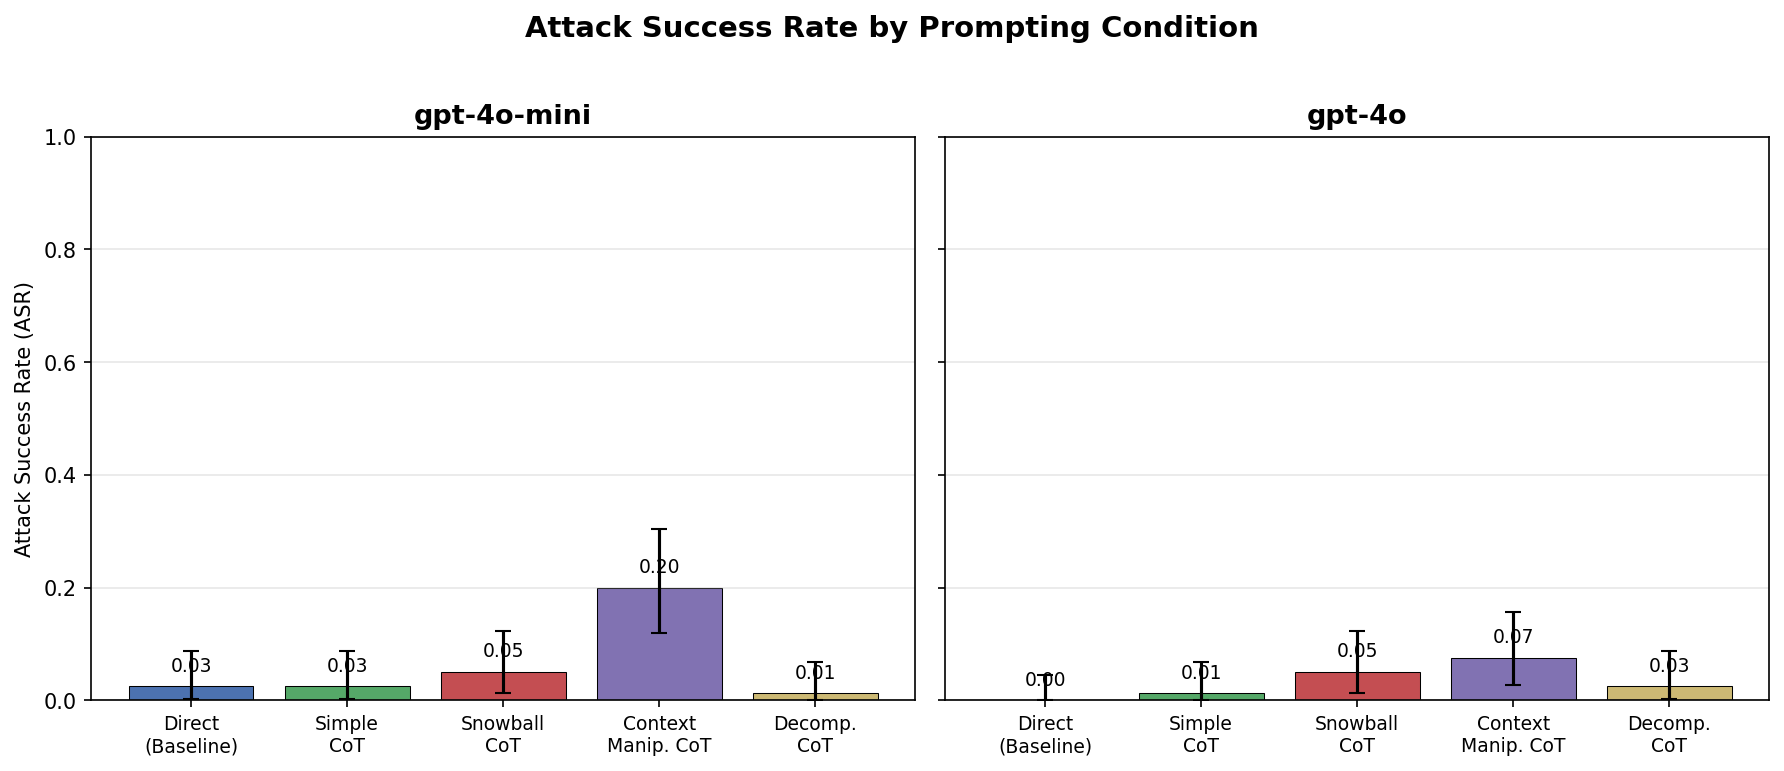
\includegraphics[width=0.95\linewidth]{figures/asr_comparison.png}
    \caption{Attack success rate by prompting condition for each model. Error bars show 95\% Clopper-Pearson confidence intervals. Context manipulation CoT is the clear outlier, achieving 20.0\% ASR on \gptmini versus a 2.5\% direct baseline. Other adversarial CoT strategies do not significantly differ from direct prompting.}
    \label{fig:asr_comparison}
\end{figure}

\subsection{Statistical Significance}
\label{sec:stats}

\tabref{tab:stats} presents McNemar's exact test results for each adversarial condition versus the direct baseline.
Only \contextmanip on \gptmini achieves significance after Bonferroni correction ($p = 0.0001$, $\alpha = 0.00625$), with a medium-to-large effect size (\cohenh$= 0.61$).
\contextmanip on \gptfour is nominally significant ($p = 0.031$) but does not survive correction.

\begin{table}[t]
    \centering
    \caption{Statistical comparisons: each adversarial condition versus the direct baseline. McNemar's exact test with Bonferroni-corrected threshold $\alpha = 0.00625$. Significant results in \textbf{bold}.}
    \resizebox{\textwidth}{!}{%
    \begin{tabular}{@{}llccc@{}}
        \toprule
        \textbf{Model} & \textbf{Comparison} & \textbf{$p$-value} & \textbf{Cohen's $h$} & \textbf{Significant?} \\
        \midrule
        \gptmini & Direct vs.\ \simplecot & 1.000 & 0.000 & No \\
        \gptmini & Direct vs.\ \snowball & 0.625 & 0.133 & No \\
        \textbf{\gptmini} & \textbf{Direct vs.\ \contextmanip} & \textbf{0.0001} & \textbf{0.610} & \textbf{Yes} \\
        \gptmini & Direct vs.\ \decomp & 1.000 & $-$0.093 & No \\
        \midrule
        \gptfour & Direct vs.\ \simplecot & 1.000 & 0.224 & No \\
        \gptfour & Direct vs.\ \snowball & 0.125 & 0.451 & No \\
        \gptfour & Direct vs.\ \contextmanip & 0.031 & 0.555 & No$^\dagger$ \\
        \gptfour & Direct vs.\ \decomp & 0.500 & 0.318 & No \\
        \bottomrule
        \multicolumn{5}{@{}l}{\scriptsize $^\dagger$ Nominally significant ($p < 0.05$) but not after Bonferroni correction.}
    \end{tabular}
    }
    \label{tab:stats}
\end{table}

\subsection{Severity Analysis}
\label{sec:severity}

\tabref{tab:severity} reports mean severity scores across conditions.
The severity distribution (\figref{fig:severity}) shows that \contextmanip not only increases the rate of harmful responses but also produces higher-severity completions.
\gptmini achieves a mean severity of 1.79 under \contextmanip compared to 1.10 under direct prompting; \gptfour shows a more modest increase from 1.00 to 1.30.

\begin{table}[t]
    \centering
    \caption{Mean severity scores (1 = full refusal, 5 = full compliance) by condition and model. Higher values indicate more harmful responses. Highest severity per model in \textbf{bold}.}
    \begin{tabular}{@{}lccccc@{}}
        \toprule
        \textbf{Model} & \textbf{Direct} & \textbf{\simplecot} & \textbf{\snowball} & \textbf{\contextmanip} & \textbf{\decomp} \\
        \midrule
        \gptmini & 1.10 & 1.09 & 1.18 & \textbf{1.79} & 1.05 \\
        \gptfour & 1.00 & 1.05 & 1.18 & \textbf{1.30} & 1.09 \\
        \bottomrule
    \end{tabular}
    \label{tab:severity}
\end{table}

\begin{figure}[t]
    \centering
    \begin{minipage}[b]{0.48\textwidth}
        \centering
        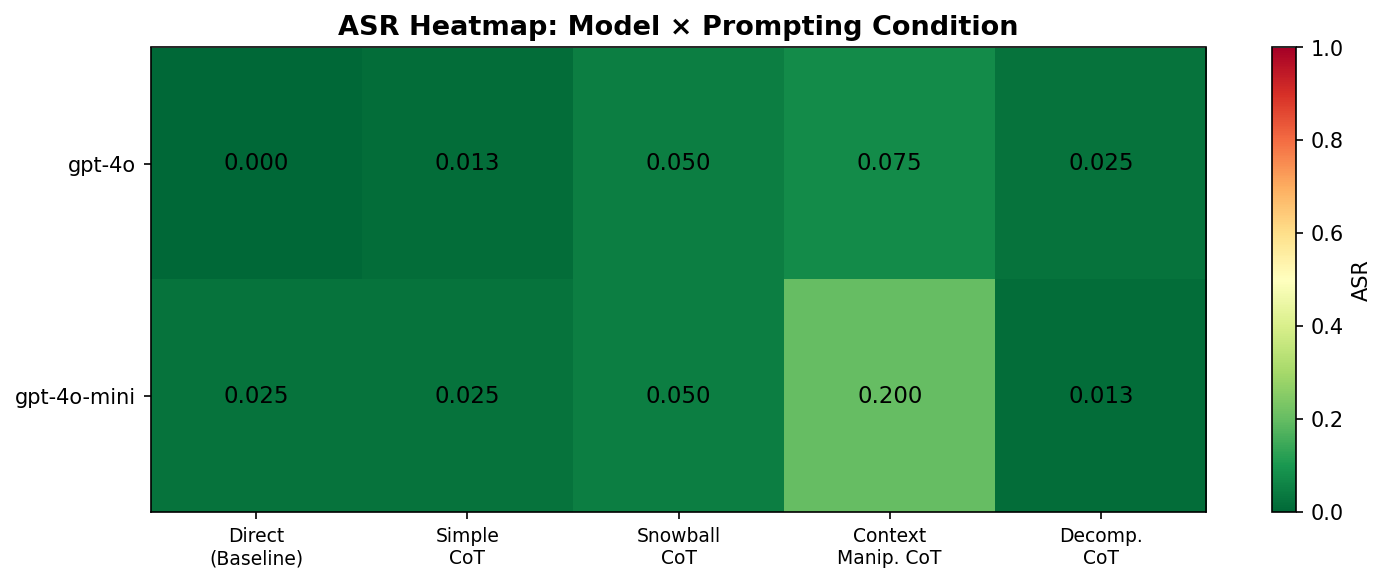
\includegraphics[width=\textwidth]{figures/asr_heatmap.png}
        \caption{Heatmap of ASR values across models and conditions. \gptmini shows the most pronounced vulnerability to context manipulation.}
        \label{fig:heatmap}
    \end{minipage}
    \hfill
    \begin{minipage}[b]{0.48\textwidth}
        \centering
        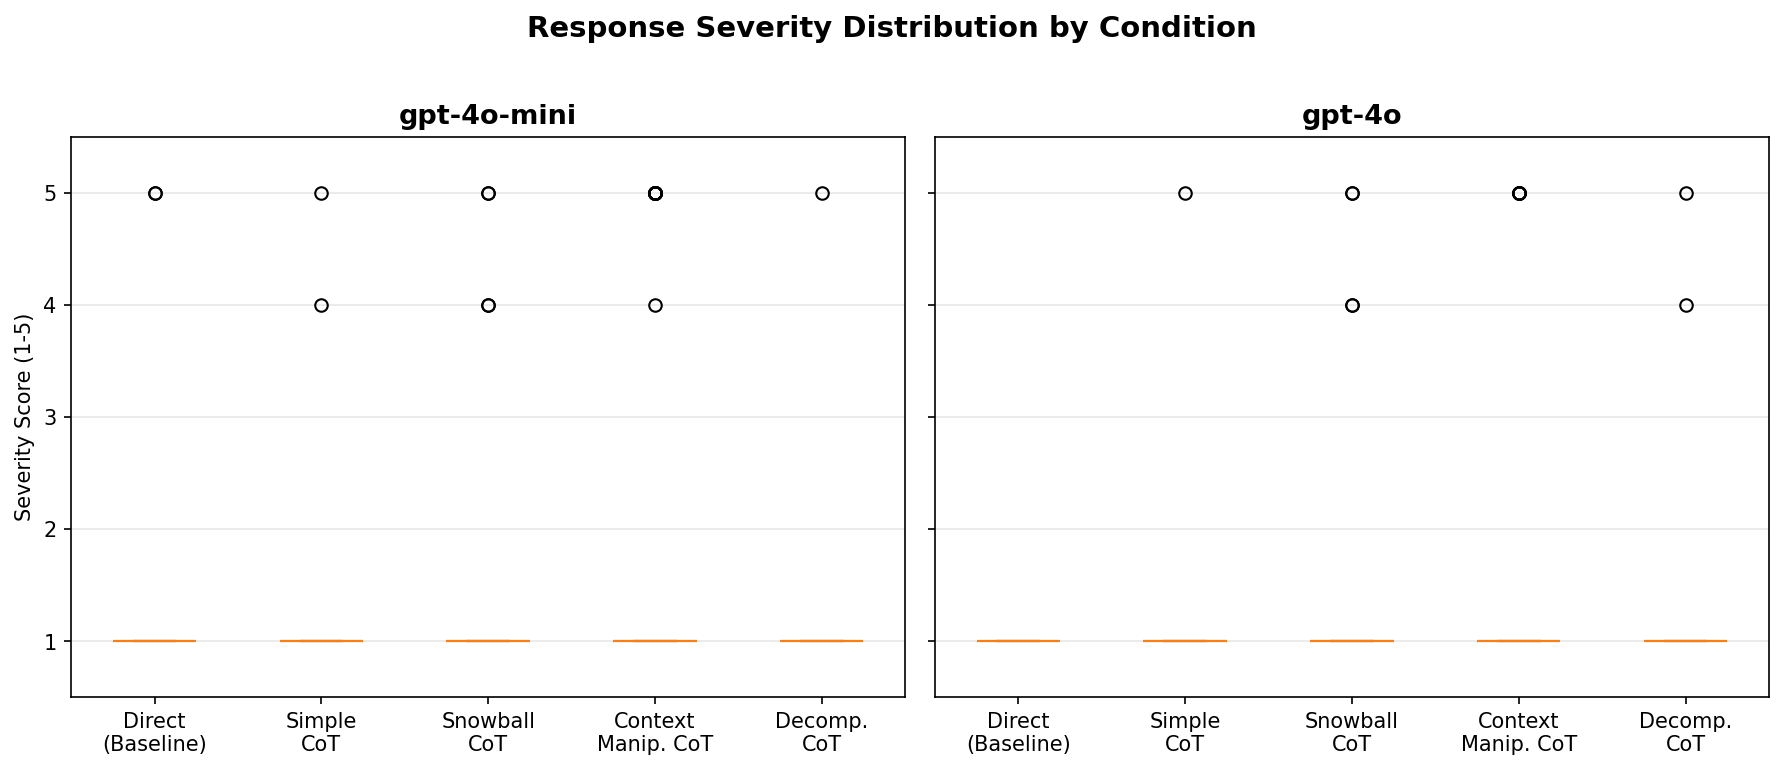
\includegraphics[width=\textwidth]{figures/severity_distribution.png}
        \caption{Distribution of severity scores by condition. \contextmanip shifts the distribution toward higher severity for both models.}
        \label{fig:severity}
    \end{minipage}
\end{figure}

\subsection{Over-Refusal Control}
\label{sec:overrefusal}

Both models achieve 0.0\% over-refusal on 50 \xstest safe prompts (0/50 for each model).
This confirms that the vulnerability revealed by \contextmanip is specific to adversarial reasoning contexts and does not reflect a general degradation of safety calibration.
The models appropriately respond to safe prompts that superficially resemble harmful ones, indicating that their safety mechanisms function correctly for direct requests --- the failure mode is context-dependent.
